\chapter{Hypatia Board}\Mynote{Überschriften nochmal anpassen}

The Hypatia Board is based on the ESP32-S3-WROOM-1 microcontroller from Espressif. It offers Wi-Fi and Bluetooth Low Energy (BLE) connectivity and can be programmed via USB. In addition to the microcontroller, the board includes the LSM100A module, which supports both LoRa and Sigfox communication standards. The Dimensions and the location of the four mounting holes are shown in the next figure\ref{fig:Dimensions}. \Mynote{Cite Hypatia Handbook} 

\begin{figure}[H]
	\centering
	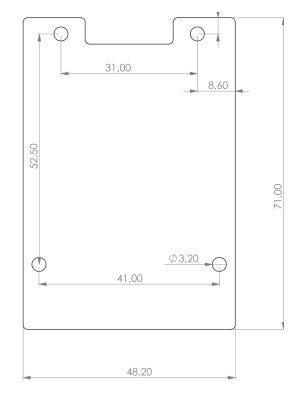
\includegraphics[width=0.3\linewidth]{../../../Images/Syde/Hypatia/Dimensions}
	\caption[Dimensions Hypatia Board]{Dimensions Hypatia Board \cite[see][1]{esp32s3wroom1:2024}}
	\label{fig:Dimensions}
\end{figure}

\section{Interface} 
The Hypatia board’s interface includes 34 female header pins for flexible peripheral connections, three JST-PH connectors for power and data interfaces, and two push buttons dedicated to reset and boot functions. Additionally, a WS2812 RGB LED provides operational feedback, enabling monitoring of the board’s status. 

\subsection{Pinout}
The board features a total of 34 female header pins.
Among these, three are connected to GND (Pins 1, 16, and 17 on J1), two provide 3.3V power (Pins 2 and 15 on J1), and one supplies 5V (Pin 17 on J2). Additionally, Pins 3 and 4 on J2 are designated for serial communication via TXD and RXD. The remaining pins serve as general-purpose input/output (GPIO). The diagram below \ref{fig:PinoutHypatia} provides a overview of which pins are safe to use, and which should be avoided or used with caution.

\begin{figure}[H]
	\centering
	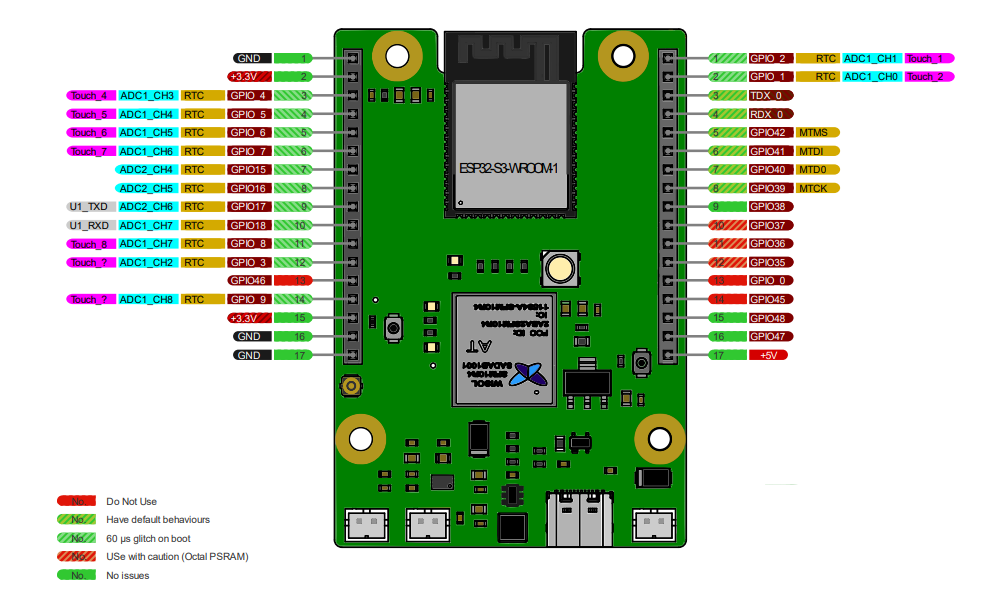
\includegraphics[width=1\linewidth]{../../../Images/Syde/Hypatia/Pinout}
	\caption[Pinout Hypatia Board]{Pinout Hypatia Board }
	\label{fig:PinoutHypatia}
\end{figure}

During the power-up phase of the ESP32-S3, certain pins may exhibit glitches, brief voltage disturbances that deviate from their normal, expected state. This happens primarily because the power rails and internal circuits require a short period to stabilize. Until the internal power domains and voltage regulators reach their steady state, the pins connected to these domains may momentarily adopt unintended logic levels. Specifically, some pins are temporarily driven low or high for approximately 60 microseconds as the chip transitions from an unpowered to a powered state. These brief glitches can be seen as a natural consequence of how the chip's internal logic and GPIO matrix handle the initial surge of power. As the system clock and internal logic gates activate and synchronize, these minor fluctuations on the pins are unavoidable. While these glitches are usually short and harmless in typical applications, designers should be aware of them, especially when connecting external components sensitive to these voltage transients. The ESP32-S3’s design accounts for these behaviors by specifying which pins experience glitches, enabling developers to plan for any potential unintended effects.

The following two tables provide information on the internal connections of the pins on either J1 or J2 to the ESP32-S3 microcontroller.

\begin{table}[!h]
\begin{center}
\caption[Pinout Hypatia Board J1]{Pinout Hypatia Board J1 \cite[see][7]{SYDE:2024}}
\label{PinoutHypatiaJ1}
\begin{tabular}{|c|c|c|}
	\hline
	\textbf{Pin J1} &\textbf{Function}  & \textbf{Description} \\
	\hline
	1& GND  & GND  \\
	\hline
	2& +3.3V  & Power supply \\
	\hline
	3& GPIO 4 & RTC\_GPIO4,GPIO4,TOUCH4,ADC1\_CH3 \\
	\hline
	4& GPIO 5 & RTC\_GPIO5,GPIO5,TOUCH5,ADC1\_CH4 \\
	\hline
	5& GPIO 6 & RTC\_GPIO6,GPIO6,TOUCH6,ADC1\_CH5 \\
	\hline
	6& GPIO 7 & RTC\_GPIO7,GPIO7,TOUCH7,ADC1\_CH6 \\
	\hline
	7& GPIO 15 & RTC\_GPIO15,GPIO15,U0RTS,ADC2\_CH4,XTAL\_32K\_P \\
	\hline
	8& GPIO 16 & RTC\_GPIO16,GPIO16,U0CTS,ADC2\_CH5,XTAL\_32K\_N \\
	\hline
	9& GPIO 17 & RTC\_GPIO17,GPIO17,U1TXD,ADC2\_CH6 \\
	\hline
	10& GPIO 18 & RTC\_GPIO18,GPIO18,U1RXD,ADC2\_CH7,CLK\_OUT3 \\
	\hline
	11& GPIO 8 & RTC\_GPIO8,GPIO8,TOUCH8,ADC1\_CH7,SUBSPICS1 \\
	\hline
	12& GPIO 3 & RTC\_GPIO3,GPIO3,TOUCH3,ADC1\_CH2 \\
	\hline
	13& GPIO 46 & GPIO46\\
	\hline
	14& GPIO 9 & RTC\_GPIO9,GPIO9,TOUCH9,ADC1\_CH8,FSPIHD,SUBSPIHD \\
	\hline
	15& +3.3V  & Power supply \\
	\hline
	16& GND  & GND  \\
	\hline
	17& GND  & GND  \\
	\hline
	\end{tabular}
	\end{center}
	\end{table}
	
	\begin{table}[!h]
	\begin{center}
		\caption[Pinout Hypatia Board J2]{Pinout Hypatia Board J2 \cite[see][8]{SYDE:2024}}
		\label{PinoutHypatiaJ1}
	\begin{tabular}{|c|c|c|}
	\hline
	\textbf{Pin J2} &\textbf{Function} & \textbf{Description} \\
	\hline
	1& GPIO 1 & RTC\_GPIO1,GPIO1, TOUCH1, ADC1\_CH0 \\
	\hline
	2& GPIO 2 & RTC\_GPIO2,GPIO2, TOUCH2, ADC1\_CH1 \\
	\hline
	3& TXD0 & RTC\_GPIO17,GPIO17,U1TXD,ADC2\_CH6 \\
	\hline
	4& RXD0  & RTC\_GPIO18,GPIO18,U1RXD,ADC2\_CH7,CLK\_OUT3 \\
	\hline
	5& GPIO 42 & MTMS,GPIO42 \\
	\hline
	6& GPIO 41 & MTDI,GPIO41, CLK\_OUT1 \\
	\hline
	7& GPIO 40 & MTDO,GPIO40,CLK\_OUT2 \\
	\hline
	8& GPIO 39 & MTCK,GPIO39,CLK\_OUT3, SUBSPICS1 \\
	\hline
	9& GPIO 38 & GPIO38,FSPIWP, SUBSPIWP \\
	\hline
	10& GPIO 37 & SPIDQS,GPIO37,FSPIQ, SUBSPIQ \\
	\hline
	11& GPIO 36 & SPIIO7,GPIO36,FSPICLK,SUBSPICLK \\
	\hline
	12& GPIO 35 & SPIIO6,GPIO35,FSPID,SUBSPID \\
	\hline
	13& GPIO 0 & RTC\_GPIO0,GPIO0 \\
	\hline
	14& GPIO 45 & GPIO45 \\
	\hline
	15& GPIO 48 & SPICLK\_N\_DIFF,GPIO48,SUBSPICLK\_N\_DIFF \\
	\hline
	16& GPIO 47 & SPICLK\_P\_DIFF,GPIO47,SUBSPICLK\_P\_DIFF \\
	\hline
	17& +5V &  \\
	\hline
\end{tabular}
\end{center}
\end{table}

\subsection{JST-PH Connectors}
A JST-PH connector is a low-profile wire-to-board connector, designed for secure and space-saving connections on high-density Printed Circuit Boards (PCBs). On the Hypatia Board three JST Connectors with 2 circuits are integrated\ref{JSTDimension}. This connector family is known for its boxed-shaped shrouded headers\cite[see][1]{JST:2024}.

\begin{figure}[H]
	\centering
	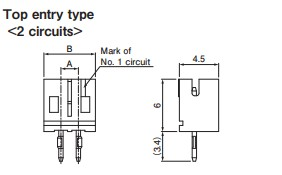
\includegraphics[width=0.3\linewidth]{../../../Images/Syde/Hypatia/JSTDimension}
	\caption[JST-PH Connector Dimension]{JST-PH Connector Dimension \cite[see][3]{JST:2024}}
	\label{fig:JSTDimension}
\end{figure}

The purpose of these three JST-PH connectors is to integrate a LiPo battery, a solar panel, and an on/off switch, enabling system reboot or reset as required, into the Hypatia circuit \ref{HypatiaSetup}. \Mynote{Add the circuit Diagramm to the switch}

\begin{figure}[H]
	\centering
	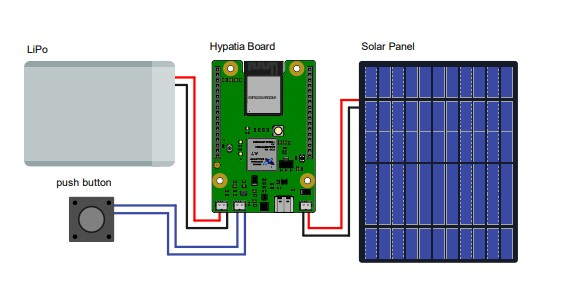
\includegraphics[width=0.7\linewidth]{../../../Images/Syde/Hypatia/HypatiaSetup}
	\caption[Setup of Hypatia Board with Lipo Battery, Solar panel and On/off Switch]{Setup of Hypatia Board with Lipo Battery, Solar panel and On/off Switch \cite[see][2]{SYDE:2024}}
	\label{fig:JSTDimension}
\end{figure}

\subsection{Boot Modus}
The Hypatia board is equipped with two push buttons: one for reset and one for boot. To upload new code to the board, it must be placed in boot mode. Boot mode is a special state that enables the microcontroller’s bootloader to receive new firmware over a serial interface. To set the board into boot mode, press and hold the reset button while briefly pressing the boot button. Once the boot button has been pressed, release both buttons. This sequence ensures that the Hypatia board is ready to accept new code uploads.
\Mynote{Tikz with button location}


\subsection{WS2812 RGB LED}
\Mynote{Check the Tables and the Text for $V_{\text{IH}}$ correct - $V_IH$ wrong}
The WS2812B is an intelligent control LED light source, seamlessly integrating a control circuit and RGB chip within a 5050 SMD package \ref{fig:WS2812BDimensions}. This compact unit features an intelligent digital data latch, a signal reshaping and amplification driver circuit, an internal oscillator, and a 12V programmable constant-current control system.
\Mynote{What is a LED, what does the control circuit, what is a 5050 SMD package. what is that data latch how does the circuit look like, explaination}
\begin{figure}[H]
	\centering
	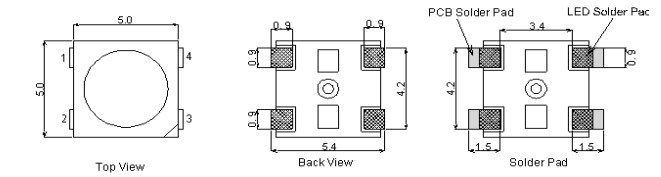
\includegraphics[width=0.7\linewidth]{../../../Images/Syde/Hypatia/WS2812BDimensions}
	\caption[Dimensions of WS2812B RGB LED]{Dimensions of WS2812B RGB LED \cite[see][2]{Worldsemi:2013}}
	\label{fig:WS2812BDimensions}
\end{figure}

The circuit of the WS2812B includes built-in reverse connection protection, preventing damage if the power supply is accidentally connected in reverse. It also incorporates an electric reset circuit and a power-loss reset circuit for reliable startup and recovery. The control circuit and the LED share a single power source, which simplifies the design and reduces component count. The Pin out and the Pin Functions are presented in the following table \ref{PinFunctionWS2812B} and visualized in the following picture \ref{WS2812BPinout}.

\begin{table}[H]
	\begin{center}
		\caption[PIN function WS2812B]{PIN function WS2812B \cite[see][2]{Worldsemi:2024}}
		\label{PinFunctionWS2812B}
		\begin{tabular}{|c|c|c|}
			\hline
			\textbf{NO.} & \textbf{Symbol} & \textbf{Function description}  \\
			\hline
			1 & VDD & Power supply LED\\
			\hline
			2 & DOUT & Control data signal output\\
			\hline
			3 & VSS & Ground\\
			\hline
			4 & DIN & Control data signal input\\
			\hline
		\end{tabular}
	\end{center}
\end{table}

\begin{figure}[H]
	\centering
	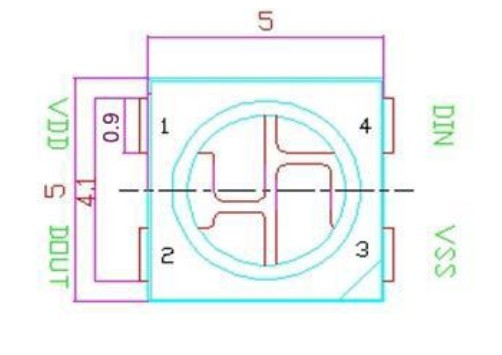
\includegraphics[width=0.7\linewidth]{../../../Images/Syde/Hypatia/WS2812BPinout}
	\caption[Pinout of WS2812B RGB LED]{Pinout of WS2812B RGB LED \cite[see][3]{Worldsemi:2024}}
	\label{fig:WS2812BPinout}
\end{figure}

The absolute maximum ratings of the WS2812B LED module specify the limits beyond which permanent damage may occur. The power supply voltage, $V_{\text{DD}}$, can range from +3.5V to +5.3V. The input voltage, $V_I$, can vary from -0.5V up to $V_{\text{DD}}$ +0.5V. The module can operate within a junction temperature range of -25\,$^\circ C$ to +80\,$^\circ C$, and can be stored safely at temperatures ranging from -40\,$^\circ C$ to +105\,$^\circ C$ \cite[see][2]{Worldsemi:2024}. 
Regarding electrical input parameters, the maximum input current ($I_IN$) is specified at $\pm1\mu A$ under typical conditions ($T_A = -20\,\mathrm{^\circ C} \sim +70\,\mathrm{^\circ C}$, $V_{DD} = 4.5\,\mathrm{V} \sim 5.5\,\mathrm{V}$, $V_{SS} = 0\,\mathrm{V}$, unless otherwise specified). For the input voltage levels, a logic high ($V_{\text{IH}}$) must be at least 0.7 times the supply voltage ($V_{\text{DD}}$), while a logic low ($V_{\text{IL}}$) must be no more than 0.3 times $V_{\text{DD}}$. The hysteresis voltage ($V_H$), which defines the difference between switching thresholds to avoid signal noise, has a typical value of 0.35V \ref{ElectrWS2812B}.

\begin{table}[H]
	\begin{center}
		\caption[Electrical Characteristics WS2812B]{Electrical Characteristics WS2812B \cite[see][3]{Worldsemi:2024}}
		\label{ElectrWS2812B}
		\begin{tabular}{|c|c|c|c|c|c|c|c|}
			\hline
			\textbf{Prameter} & \textbf{Smybol} & \textbf{conditions} & \textbf{Min} & \textbf{Tpy} & \textbf{Max} & \textbf{Unit} \\
			\hline
			Input current & $I_I$ & $V_I = V_{\text{DD}}/V_{\text{SS}}$ & & &$\pm 1$ & $\mu A$\\ \hline
			\multirow{ 2}{*}{Input voltage level} & $V_{\text{IH}}$ & $D_IN$, SET & 0.7$V_{\text{DD}}$ & & & V\\ \cline{2-7}
			& $V_{\text{IL}}$ & $D_IN$, SET & & & 0.3 $V_{\text{DD}}$ & V\\ \hline
			Hysteresis voltage & $V_H$ & $D_IN$, SET &  & 0.35 &  & V\\ \hline
		\end{tabular}
	\end{center}
\end{table}

\subsubsection{Data transmission}
The WS2812B supports transmission distances of more than 5 meters between any two points without the need for additional circuitry. At a refresh rate of 30 frames per second, it supports a cascade length of at least 1024 pixels. Data transmission speeds reach up to 800\,Kbps \cite[see][2]{Worldsemi:2024}.

To ensure reliable communication between the microcontroller or data source and the WS2812B, regardless of how many LEDs are in the chain, the protocol specifies a bit period of 1.25\,$\mu$s (with a margin of $\pm$600\,ns), and each bit is represented by a distinct high and low voltage timing pattern \ref{fig:SequTimeWS2812B}. 

\begin{figure}[H]
	\centering
	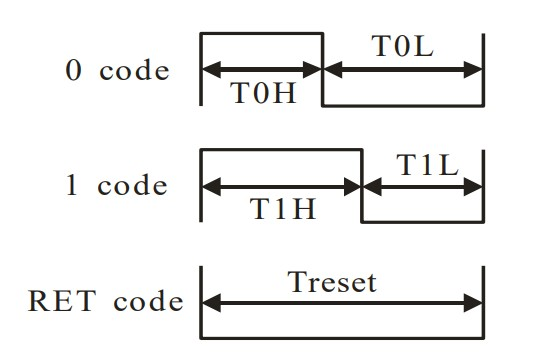
\includegraphics[width=0.5\linewidth]{../../../Images/Syde/Hypatia/SequTimeWS2812B}
	\caption[Sequence Times WS2812B]{Sequence Times WS2812B \cite[see][4]{JST:2024}}
	\label{fig:SequTimeWS2812B}
\end{figure}

The precise high and low voltage durations for transmitting logical ‘0’ and ‘1’ bits, as well as the reset condition are provided by the following table\ref{WS2812BTransferTime}.

\begin{table}[H]
	\begin{center}
		\caption[Data transfer time for WS2812B]{Data transfer time for WS2812B (TH+TL=1.25\,$\mu$s$\pm$600\,ns) \cite[see][3]{Worldsemi:2024}}
		\label{WS2812BTransferTime}
		\begin{tabular}{|c|c|c|c|}
			\hline
			\textbf{Symbol} & \textbf{Description} & \textbf{Typical} & \textbf{Tolerance} \\
			\hline
			TOH & 0 code, high voltage time & 0.4\,$\mu$s & $\pm$150\,ns \\
			\hline
			T1H & 1 code, high voltage time & 0.8\,$\mu$s & $\pm$150\,ns \\
			\hline
			T0L & 0 code, low voltage time & 0.85\,$\mu$s & $\pm$150\,ns \\
			\hline
			T1L & 1 code, low voltage time & 0.45\,$\mu$s & $\pm$150\,ns \\
			\hline
			RES & Low voltage time & Above 50\,$\mu$s &\\
			\hline
		\end{tabular}
	\end{center}
\end{table}

For a ‘0’ bit (shown as “0 code” in the diagram), the data line is held high for 0.4\,$\mu$s (T0H) and then low for 0.85\,$\mu$s (T0L). This combination of a short high period followed by a longer low period defines the ‘0’ bit and allows the LED to interpret it correctly.

For a ‘1’ bit (shown as “1 code”), the data line is held high for a longer period of 0.8\,$\mu$s (T1H), followed by a shorter low period of 0.45\,$\mu$s (T1L). This pattern of a longer high time and a shorter low time distinguishes the ‘1’ bit from the ‘0’ bit.

The final diagram shows the reset code (RET code). Here, the data line is held low for a minimum of 50 microseconds (Treset). This low voltage period is significantly longer than the timing for individual data bits and signals to all LEDs that a new data transmission cycle will begin. This reset code ensures that all LEDs are synchronized to receive the next series of color data.

\begin{table}[H]
	\begin{center}
		\caption[Switching characteristics of the WS2812B]{Switching characteristics of the WS2812B \cite[see][3]{Worldsemi:2024}}
		\label{SwitchingTimeWS2812B}
		\begin{tabular}{|c|c|c|c|c|c|c|}
			\hline
			\textbf{Parameter} & \textbf{Symbol} & \textbf{Condition} & \textbf{Min} & \textbf{Typ} & \textbf{Max} & \textbf{Unit} \\
			\hline
			Transmission delay  & \multirow{2}{*}{$t_{PLZ}$ }& CL=15pF, DIN$\rightarrow$& & & \multirow{2}{*}{300} & \multirow{2}{*}{ns} \\
			time & & DOUT, RL=10k$\Omega$ & & & & \\
			\hline
			\multirow{2}{*}{Fall time} & \multirow{2}{*}{$t_{THZ}$} & CL=300pF, & & & \multirow{2}{*}{120} & \multirow{2}{*}{$\mu$s} \\
			& & OUTR/OUTG/OUTB & & & & \\
			\hline
			Input capacity & $C_1$ & & & & 15 & pF \\
			\hline
		\end{tabular}
	\end{center}
\end{table}
\Mynote{Make the Caption of all the Tables nicer and more accurate }
In addition to the carefully defined data transfer timings for each bit (‘0’ and ‘1’ codes) and the reset condition, the switching characteristics of the WS2812B also play a role in ensuring reliable operation \ref{SwitchingTimeWS2812B}. These characteristics describe the electrical behavior of the data input and output pins, which directly influences how accurately the LEDs can interpret the incoming data signals. The transmission delay time (tPLZ), which ensures that the data stream propagates quickly from one LED to the next in the chain, amounts to 300\,ns. The fall time (tTHZ) determines how quickly the data output can transition between logic levels and is specified as 120\,$\mu$s for the WS2812B. Finally, the input capacitance (C1) indicates how much electrical load the data input pin of each LED represents, and for this RGB LED, it is 15\,pF.

\begin{figure}[H]
	\centering
	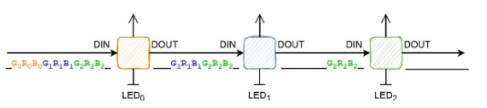
\includegraphics[width=0.7\linewidth]{../../../Images/Syde/Hypatia/SerialDataTransmissionWS2812B}
	\caption[Serial Data transmission between LEDs WS2812B]{Serial Data transmission between LEDs WS2812B \cite[see][211]{Ritschel:2023}}
	\label{fig:SerialDataTransmissionWS2812B}
\end{figure}


The diagram \ref{fig:SerialDataTransmissionWS2812B} illustrates the data transmission method of the WS2812B RGB LEDs, which operates based on a single data line. Each LED receives data through the data input pin (DIN), and the data output pin (DOUT) of one LED is connected to the DIN of the next LED in the chain. Data transmission begins with the reset code that marks the start of a new data refresh cycle. In a data refresh cycle, the data for each LED is transmitted sequentially\ref{fig:DataTransmissionWS2812B} \cite[see][211]{Worldsemi:2013}.\Mynote{How to do the citation here???! Its discribed in the picture from the datasheet not mentioned in the text from Ritschel}

\begin{figure}[H]
	\centering
	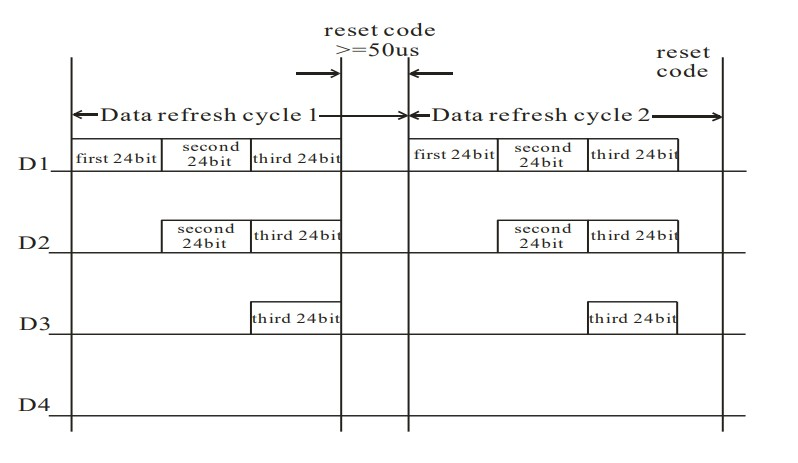
\includegraphics[width=0.7\linewidth]{../../../Images/Syde/Hypatia/DataTransmissionWS2812B}
	\caption[Data transmission method WS2812B]{Data transmission method WS2812B \cite[see][4]{Worldsemi:2024}}
	\label{fig:DataTransmissionWS2812B}
\end{figure}

Each LED requires 24-bit color data, split into 8 bits for green, 8 bits for red, and 8 bits for blue. These data packets are transmitted in succession and determine the brightness and color of each LED. After a pause, the RGB data is transmitted cyclically to all LEDs. The first LED receives the first 24-bit RGB data and then forwards the remaining data stream to the next LED, which also takes its own 24-bit data and forwards the rest. This approach ensures that each LED receives its unique data \ref{fig:DataTransmissionWS2812B} \cite[see][211]{Ritschel:2023}.

Once the data for all LEDs has been transmitted, another reset code (a low signal for at least 50 microseconds) ends the current refresh cycle and prepares the LEDs for the next update. This cycle repeats whenever new color data needs to be sent to the LEDs \ref{fig:DataTransmissionWS2812B}.

\subsubsection{RGB characteristics}
Each pixel, made up of the three primary colors (red, green, and blue \ref{RGBWS2812B}), supports 256 levels of brightness per channel. This allows the WS2812B to achieve a full-color display with 16.777.216 possible colors and a scan frequency of at least 400 Hz per second.

\begin{table}[H]
	\begin{center}
		\caption[RGB IC characteristic parameter WS2812B]{RGB IC characteristic parameter WS2812B \cite[see][3]{Worldsemi:2024}}
		\label{RGBWS2812B}
		\begin{tabular}{|c|c|c|c|c|}
			\hline
			\textbf{Emitting color} & \textbf{Model} & \textbf{Wavelength} & \textbf{Luminous intensity} & \textbf{Voltage}\\
			\hline
			\textcolor{red}{Red} & 13CBAUP & 620-625\,nm & 390-420\,mcd & 2.0-2.2\,V\\
			\hline
			\textcolor{green}{Green} & 13CGAUP & 522-525\,nm & 660-720\,mcd & 3.0-3.4\,V\\
			\hline
			\textcolor{blue}{Blue} & 10R1MUX & 465-467\,nm & 180-200\,mcd & 3.0-3.4\,V\\
			\hline
		\end{tabular}
	\end{center}
\end{table}

\subsubsection{\FILE{Adafruit\_NeoPixel Library}}
\Mynote{Find any discribtion of Library -Git doesnt work}
The Adafruit DMA NeoPixel library, version 1.3.3, released on April 24, 2024, and published under the MIT license is specifically designed for NeoPixel DMA support on SAMD21 and SAMD51 microcontrollers using the Arduino platform and is maintained by Adafruit. 

\subsubsection{\FILE{WS2812B Example Code} for Hypatia}

The Hypatia Handbook provides example code to test the WS2812B RGB LED using the Adafruit NeoPixel library \ref{lst:WS2812BExample}. Utilizing GPIO21 for data transmission within the Arduino environment, the code controls the LED to alternately glow red, green, and blue, changing every 50\,ms \cite[see][12]{SYDE:2024}.

\definecolor{codegreen}{rgb}{0,0.6,0}
\definecolor{codegray}{rgb}{0.5,0.5,0.5}
\definecolor{codepurple}{rgb}{0.58,0,0.82}
\definecolor{backcolour}{rgb}{0.95,0.95,0.92}

\lstinputlisting[
caption= \FILE{WS2812B Example Code},
label={lst:WS2812BExample},
language=C++,
backgroundcolor=\color{backcolour},   
commentstyle=\color{codegreen},
keywordstyle=\color{magenta},
numberstyle=\tiny\color{codegray},
stringstyle=\color{codepurple},
basicstyle=\ttfamily\footnotesize,
breakatwhitespace=false,         
breaklines=true,                 
keepspaces=true,                 
numbers=left,       
numbersep=5pt,                  
showspaces=false,                
showstringspaces=false,
showtabs=false,                  
tabsize=2]{../../Code/Syde/HTADemonstrator/Test/TestWS2812/TestWS2812.ino}



The code begins by including the \FILE{Adafruit\_NeoPixel Library}, which provides functions to control the LED. The \PYTHON{LED\_PIN} is set to 21, specifying the pin on the microcontroller to which the data input of the WS2812B LED is connected. \PYTHON{NUM\_LEDS} is defined as 1, indicating that only a single LED is in use. An NeoPixel Object of the \PYTHON{Adafruit\_NeoPixel} class, named \PYTHON{strip}, is created with parameters specifying the number of LEDs, the data pin, and the LED color order and protocol speed (\PYTHON{NEO\_GRB }+ \PYTHON{NEO\_KHZ800}). This combination tells the library to use green, red, and blue as the order for the color data and to communicate at 800\,kHz, matching the WS2812B’s protocol. The \PYTHON{setup()} function runs once when the microcontroller is powered up or reset. Here, strip.begin() initializes the LED data pin and prepares the NeoPixel library for communication. The call to \PYTHON{strip.show()} ensures that the LED is initially turned off by updating the LED with any pending color changes (which, at this point, are off by default). The \PYTHON{loop()} function runs continuously after \PYTHON{setup()} finishes. In this loop, the LED color is changed to red by calling \PYTHON{strip.setPixelColor(0, strip.Color(255, 0, 0))}, which sets the LED’s color to full red with no green or blue. \PYTHON{strip.show()} is called immediately afterward to send the color data to the LED, making the LED light up red. A short \PYTHON{delay(50)} is inserted to keep the LED red for 50\,ms. The same process is repeated for green and blue colors. \PYTHON{strip.setPixelColor(0, strip.Color(0, 255, 0))} changes the LED to green, and after 50\,ms, \PYTHON{strip.setPixelColor(0, strip.Color(0, 0, 255))} changes it to blue. 

\section{ESP32-S3-WROOM-1}
The ESP32-S3-WROOM-1 module is an integrated wireless and microcontroller platform designed for a wide range of embedded applications. It features 2.4\,GHz Wi-Fi (802.11b/g/n) and Bluetooth 5 connectivity and is based on the ESP32-S3 series of SoCs, which incorporate a dual-core 32-bit Xtensa LX7 microprocessor. The module supports up to 16\,MB of flash and 16\,MB of PSRAM, and provides up to 36 GPIOs along with a comprehensive set of digital and analog peripherals and wireless communication is enabled through an on-board PCB antenna.


\begin{figure}[H]
	\centering
	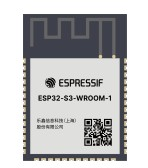
\includegraphics[width=0.3\linewidth]{../../../Images/Syde/Hypatia/ESP32S3}
	\caption[ESP32-S3-WROOM-1]{ESP32-S3-WROOM-1 \cite[see][1]{Espressif:2024}}
	\label{fig:ESP32}
\end{figure}

\subsection{Physical Dimensions}
Figure \ref{fig:espDimensions} shows the ESP32-S3-WROOM-1 module with dimensions in millimeters. The module measures 18.0\,mm in width and 25.5\,mm in length, with a maximum height of 3.1\,mm including the shielding. Pin pads are arranged along the sides with a standard pitch of 1.27\,mm, while the central pad area on the bottom side measures 7.5\,mm $\times$10.29\,mm. The top view includes antenna placement and keep-out zones, while the bottom view indicates pad layout and spacing relevant for PCB footprint design. Tolerances are specified for key dimensions to support accurate mechanical integration.

\begin{figure}[H]
	\centering
	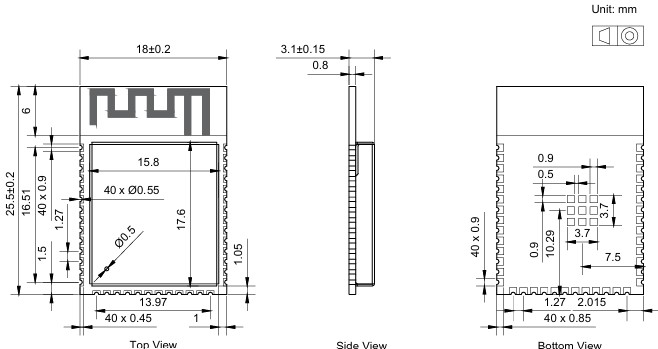
\includegraphics[width=0.7\linewidth]{../../../Images/Syde/Hypatia/espDimensions}
	\caption[ESP32-S3-WROOM-1]{ESP32-S3-WROOM-1 \cite[see][9]{Espressif:2024}}
	\label{fig:espDimensions}
\end{figure}

\subsection{Block Diagramm}
The diagrams illustrate the block structure of the ESP32-S3-WROOM-1 module. Power is supplied via a 3.3\,V line. A 40\,MHz crystal oscillator provides a stable timing reference for the system. The module incorporates an RF matching circuit connected to an antenna for wireless communications. It also integrates a Quad SPI (QSPI) flash memory interface, which supports optional PSRAM. Several SPI signals, including SPICSO, SPICLK, SPIQ, SPID, SPIWP, and SPIHD, are connected to the QSPI flash interface.
The module exposes general-purpose input/output (GPIO) pins for external device interfacing. A dedicated enable (EN) pin allows control of the module's power state.

\begin{figure}[H]
	\centering
	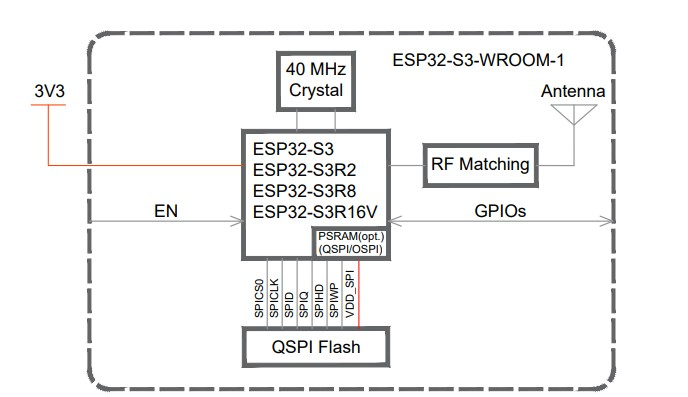
\includegraphics[width=0.7\linewidth]{../../../Images/Syde/Hypatia/ESP32S3BlockDiagramm}
	\caption[ESP32-S3-WROOM-1 Block Diagramm]{ESP32-S3-WROOM-1 Block Diagramm \cite[see][9]{Espressif:2024}}
	\label{fig:ESP32S3BlockDiagramm}
\end{figure}

\subsection{Pin Definitions}
 The module has 41 pins. The Pin Definitions are described in the following Table \ref{PinESP}.
 
\begin{longtable}[H]{|c|c|c|p{7cm}|}
	\caption[Pin Definitions of the ESP32-S3-WROOM-1]{Pin Definitions of the ESP32-S3-WROOM-1 \cite[see][3]{Espressif:2024}}
	\label{PinESP} \\
	\hline
	\textbf{Name} & \textbf{No.} & \textbf{$Type^a$} & \textbf{Function} \\
	\hline
	\endfirsthead
	
	\hline
	\textbf{Name} & \textbf{No.} & \textbf{$Type^a$} & \textbf{Function} \\
	\hline
	\endhead
	
	\hline
	\multicolumn{4}{r}{\textit{Continued on next page}} \\
	\endfoot
	
	\hline
	\endlastfoot
	
	GND & 1 & P & GND \\
	\hline
	EN & 3 & I & High: on, enables the chip. Low: off, the chip powers off. Note: Do not leave the EN pin floating. \\
	\hline
	IO4 & 4 & I/O/T & RTC\_GPIO4, \textbf{GPIO4}, TOUCH4, ADC1\_CH3 \\
	\hline
	IO5 & 5 & I/O/T & RTC\_GPIO5, \textbf{GPIO5}, TOUCH5, ADC1\_CH4 \\
	\hline
	IO6 & 6 & I/O/T & RTC\_GPIO6, \textbf{GPIO6}, TOUCH6, ADC1\_CH5 \\
	\hline
	IO7 & 7 & I/O/T & RTC\_GPIO7, \textbf{GPIO7}, TOUCH7, ADC1\_CH6 \\
	\hline
	IO15 & 8 & I/O/T & RTC\_GPIO15, \textbf{GPIO15}, U0RTS, ADC2\_CH4, XTAL\_32K\_P \\
	\hline
	IO16 & 9 & I/O/T & RTC\_GPIO16, \textbf{GPIO16}, U0CTS, ADC2\_CH5, XTAL\_32K\_N \\
	\hline
	IO17 & 10 & I/O/T & RTC\_GPIO17, \textbf{GPIO17}, U1TXD, ADC2\_CH6 \\
	\hline
	IO18 & 11 & I/O/T & RTC\_GPIO18, \textbf{GPIO18}, U1RXD, ADC2\_CH7, CLK\_OUT3 \\
	\hline
	IO8 & 12 & I/O/T & RTC\_GPIO8, \textbf{GPIO8}, TOUCH8, ADC1\_CH7, SUBSPICS1 \\
	\hline
	IO19 & 13 & I/O/T & RTC\_GPIO19, GPIO19, U1RTS, ADC2\_CH8, CLK\_OUT2, \textbf{USB\_D-} \\
	\hline
	IO20 & 14 & I/O/T & RTC\_GPIO20, GPIO20, U1CTS, ADC2\_CH9, CLK\_OUT1, \textbf{USB\_D+} \\
	\hline
	IO3 & 15 & I/O/T & RTC\_GPIO3, \textbf{GPIO3}, TOUCH3, ADC1\_CH2 \\
	\hline
	IO46 & 16 & I/O/T & \textbf{GPIO46} \\
	\hline
	IO9 & 17 & I/O/T & RTC\_GPIO9, \textbf{GPIO9}, TOUCH9, ADC1\_CH8, FSPIHD, SUBSPIHD \\
	\hline
	IO10 & 18 & I/O/T & RTC\_GPIO10, \textbf{GPIO10}, TOUCH10, ADC1\_CH9, FSPICS0, FSPIIO4, SUBSPICS0 \\
	\hline
	IO11 & 19 & I/O/T & RTC\_GPIO11, \textbf{GPIO11}, TOUCH11, ADC2\_CH0, FSPID, FSPIIO5, SUBSPID \\
	\hline
	IO12 & 20 & I/O/T & RTC\_GPIO12, \textbf{GPIO12}, TOUCH12, ADC2\_CH1, FSPICLK, FSPIIO6, SUBSPICLK \\
	\hline
	IO13 & 21 & I/O/T & RTC\_GPIO13, \textbf{GPIO13}, TOUCH13, ADC2\_CH2, FSPIQ, FSPIIO7, SUBSPIQ \\
	\hline
	IO14 & 22 & I/O/T & RTC\_GPIO14, \textbf{GPIO14}, TOUCH14, ADC2\_CH3, FSPIWP, FSPIDQS, SUBSPIWP \\
	\hline
	IO21 & 23 & I/O/T & RTC\_GPIO21, \textbf{GPIO21} \\
	\hline
	IO47$^c$ & 24 & I/O/T & SPICLK\_P\_DIFF, \textbf{GPIO47}, SUBSPICLK\_P\_DIFF \\
	\hline
	IO48$^c$ & 25 & I/O/T & SPICLK\_N\_DIFF, \textbf{GPIO48}, SUBSPICLK\_N\_DIFF \\
	\hline
	IO45 & 26 & I/O/T & \textbf{GPIO45} \\
	\hline
	IO0 & 27 & I/O/T & RTC\_GPIO0, \textbf{GPIO0} \\
	\hline
	IO35$^b$ & 28 & I/O/T & SPIIO6, \textbf{GPIO35}, FSPID, SUBSPID \\
	\hline
	IO36$^b$ & 29 & I/O/T & SPIIO7, \textbf{GPIO36}, FSPICLK, SUBSPICLK \\
	\hline
	IO37$^b$ & 30 & I/O/T & SPIDQS, \textbf{GPIO37}, FSPIQ, SUBSPIQ \\
	\hline
	IO38 & 31 & I/O/T & \textbf{GPIO38}, FSPIWP, SUBSPIWP \\
	\hline
	IO39 & 32 & I/O/T & \textbf{MTCK}, GPIO39, CLK\_OUT3, SUBSPICS1 \\
	\hline
	IO40 & 33 & I/O/T & \textbf{MTDO}, GPIO40, CLK\_OUT2 \\
	\hline
	IO41 & 34 & I/O/T & \textbf{MTDI}, GPIO41, CLK\_OUT1 \\
	\hline
	IO42 & 35 & I/O/T & \textbf{MTMS}, GPIO42 \\
	\hline
	RXD0 & 36 & I/O/T & \textbf{U0RXD}, GPIO44, CLK\_OUT2 \\
	\hline
	TXD0 & 37 & I/O/T & \textbf{U0TXD}, GPIO43, CLK\_OUT1 \\
	\hline
	IO2 & 38 & I/O/T & RTC\_GPIO2, \textbf{GPIO2}, TOUCH2, ADC1\_CH1 \\
	\hline
	IO1 & 39 & I/O/T & RTC\_GPIO1, \textbf{GPIO1}, TOUCH1, ADC1\_CH0 \\
	\hline
	GND & 40 & P & GND \\
	\hline
	EPAD & 41 & P & GND \\
	\hline
\end{longtable}

The table includes extra pin functions for the ESP32-S3:
\begin{itemize}
	\item $^a$: Pin roles are denoted using the following abbreviations: P for power supply, I for input, O for output, and T for high impedance. Default functions are shown in bold font. For pins 28 to 30, the default function depends on the configuration of the eFuse bit.
	 \item $^b$: For modules equipped with Octal SPI PSRAM (such as the ESP32-S3R8 or ESP32-S3R16V), pins IO35, IO36, and IO37 are internally connected to the memory and cannot be repurposed.
	 \item $^c$: Additionally, on ESP32-S3R16V modules, GPIO47 and GPIO48 operate at 1.8\,V, as determined by the VDD\_SPI voltage of the chip. This voltage level differs from the standard operating voltage of other GPIOs on the device.
\end{itemize} 

\subsection{Boot Configurations}
At startup or following a hardware reset, the ESP32-S3 chip automatically configures several boot parameters using a combination of strapping pins and eFuse bits, without requiring any input from the microcontroller. The boot mode is determined by the state of GPIO0 and GPIO46, while the VDD\_SPI voltage level is set via GPIO45 or by programming the eFuse bits EFUSE\_VDD\_SPI\_FORCE and EFUSE\_VDD\_SPI\_TIEH. Similarly, control over ROM message printing is handled through GPIO46 and can also be managed using the eFuse settings EFUSE\_UART\_PRINT\_CONTROL and EFUSE\_DIS\_USB\_SERIAL\_JTAG\_ROM\_PRINT. The JTAG signal source is selected using GPIO3, with additional configuration options provided by the eFuses EFUSE\_DIS\_PAD\_JTAG, EFUSE\_DIS\_USB\_JTAG, and EFUSE\_STRAP\_JTAG\_SEL. All of these eFuse parameters are initially set to zero, indicating they are unprogrammed. Since eFuses are one-time programmable, setting any of these bits to one is permanent and cannot be reversed. 

\paragraph{Chip Boot Mode Control} The boot mode of the ESP32-S3 is determined by the states of GPIO0 and GPIO46 after reset. If GPIO0 is high, the device enters SPI Boot mode, which is the default configuration, allowing the ROM bootloader to load and execute code directly from the SPI flash. If both GPIO0 and GPIO46 are low, the chip enters Joint Download Boot mode, which supports multiple download methods including USB Download Boot via USB-Serial/JTAG or USB-OTG, as well as UART Download Boot. In this mode, users can transfer binary files into flash memory or SRAM using a UART or USB interface. Additionally, the ESP32-S3 supports SPI Download Boot mode as an alternative. 

\paragraph{VDD\_SPI Voltage Control} The VDD\_SPI voltage on the ESP32-S3 can be configured using GPIO45 and eFuse settings, depending on the value of EFUSE\_VDD\_SPI\_FORCE. By default, the voltage is set to 3.3\,V through the RTC domain. If custom voltage levels are needed, such as 1.8\,V from the flash regulator, this can be enabled by setting the relevant eFuse bits. The eFuse settings EFUSE\_VDD\_SPI\_FORCE and EFUSE\_VDD\_SPI\_TIEH determine whether the source and level of VDD\_SPI are fixed or software-configurable.

\paragraph{ROM Messages Printing Control} During boot, ROM messages from the chip can be printed to different interfaces. By default, output is directed to the UART0 or the USB Serial/JTAG controller. This behavior can be modified by setting specific eFuse bits or adjusting registers, allowing the messages to be redirected to either UART0 or USB, depending on system needs.

\paragraph{JTAG Signal Source Control} The JTAG signal source on the ESP32-S3 can be configured during early boot using the strapping pin GPIO3 in combination with several eFuse settings. Since GPIO3 lacks internal pull resistors, its strapping state must be externally controlled and must not be left floating. Depending on the configuration of EFUSE\_DIS\_PAD\_JTAG, EFUSE\_DIS\_USB\_JTAG, and EFUSE\_STRAP\_JTAG\_SEL, JTAG signals can be routed either to the USB Serial/JTAG controller or to the dedicated JTAG pins (MTDI, MTCK, MTMS, MTDO). If required, JTAG functionality can also be completely disabled by setting the appropriate eFuses.

\subsection{Peripherals}
The ESP32-S3 features a range of integrated peripherals including interfaces such as SPI, UART, I2C, I2S, LCD, camera, and SD/MMC, as well as functional modules like LED PWM, pulse counter, remote control, and USB Serial/JTAG. The chip also supports motor control (MCPWM), analog input (ADC), capacitive touch, and temperature sensing. Additionally, it integrates a full-speed USB 2.0 OTG interface for direct USB communication and includes a TWAI® controller, which is compatible with CAN Specification 2.0 (ISO 11898-1).

\subsubsection{Connectivity Interface}
The connectivity interfaces on the chip enable communication and interaction with external devices and networks.

\paragraph{UART Controller}
Three UART controllers—UART0, UART1, and UART2—designed for high-speed, full-duplex asynchronous communication are included in the ESP32-S3. Supporting speeds up to 5\,Mbps, these controllers are compatible with RS232, RS485, and IrDA protocols. Each UART shares a common 1024 x 8-bit RAM for transmit (TX) and receive (RX) FIFOs and offers features like programmable baud rate, automatic baud rate detection, special character detection (AT\_CMD), hardware/software flow control, and GDMA support for high-speed data transfers. UARTs can also be used as a wake-up source from low-power states. In terms of pin assignments, UART0 and UART1 use fixed GPIOs by default but can be mapped to any GPIO via the GPIO Matrix. UART0 transmit (U0TXD) and receive (U0RXD) are multiplexed with GPIO43 and GPIO44, while flow control pins (U0RTS/U0CTS and U0DTR/U0DSR) can also be routed through various GPIOs. Similarly, UART1 uses GPIO17 and GPIO18 for TX/RX and GPIO19 and GPIO20 for RTS/CTS, but again, all signals can be reassigned via the GPIO Matrix. UART2 offers complete flexibility, allowing all its signals to be mapped freely to any GPIO.

\paragraph{I2C Interface}
The ESP32-S3 features two I2C bus interfaces that can operate in either master or slave mode, depending on the application. It supports standard mode (100\,kbit/s), fast mode (400\,kbit/s), and speeds up to 800\,kbit/s, limited by the strength of the pull-up resistors on the SCL and SDA lines. Both 7-bit and 10-bit addressing modes are available, with support for double addressing (slave and register addressing). The hardware includes a command abstraction layer to simplify I2C usage. I2C pins can be mapped to any GPIO via the GPIO Matrix, offering flexible pin configuration.

\paragraph{I2S Interface}
Integrated are two standard I2S interfaces that support both master and slave modes, as well as full-duplex or half-duplex communication. These interfaces are configurable, allowing for 8-, 16-, 24-, or 32-bit data resolution for both input and output channels. They support BCK clock frequencies ranging from 10\,kHz to 40\,MHz and include a dedicated DMA controller. The I2S interface is compatible with TDM PCM, TDM MSB/LSB alignment, TDM Phillips, and PDM formats. Like other peripherals, I2S signals can be mapped to any GPIO using the GPIO Matrix.

\paragraph{LCD and Camera Controller}
A LCD and camera controller enables efficient handling of parallel video data streams. The LCD module supports 8- to 16-bit parallel RGB, I8080, and MOTO6800 interfaces, with operating speeds up to 40\,MHz. It includes built-in support for format conversion between RGB565, YUV422, YUV420, and YUV411. On the input side, the camera module is designed to interface with DVP image sensors over an 8- to 16-bit parallel bus, also running at frequencies up to 40\,MHz. It offers the same range of video format conversions as the LCD module. Pin assignments for both interfaces are flexible and can be configured using the GPIO Matrix.

\paragraph{Serial Peripheral Interface (SPI)}
The ESP32-S3 provides a versatile and high-performance Serial Peripheral Interface (SPI) system consisting of four separate SPI controllers: SPI0, SPI1, SPI2, and SPI3. SPI0 and SPI1 are primarily reserved for internal operations, such as communication with flash memory and PSRAM, and are typically not used for general-purpose peripheral control. SPI2 and SPI3, on the other hand, are designed as flexible general-purpose SPI interfaces and can be configured as needed. Both SPI2 and SPI3 support single, dual, quad, and octal SPI communication, offering compatibility with a broad range of external devices. These interfaces allow operation in both master and slave modes, and support full-duplex and half-duplex data transfers. Clock frequencies can be set up to 80\,MHz in SDR (single data rate) mode and up to 40\,MHz in DDR (double data rate) mode, with full configurability of clock polarity (CPOL) and phase (CPHA), providing fine-grained control over signal timing. Data can be transmitted in bytes, with selectable bit order (MSB first or LSB first). Furthermore, SPI2 and SPI3 support DMA (via GDMA) for high-speed, low-latency data transfers without CPU intervention. SPI2 additionally offers connection to up to six independent SPI slaves, with configurable chip-select (CS) setup time and hold time. When acting as a master, SPI2 can support 2-, 4-, or 8-line half-duplex communication and 2-line full-duplex communication, depending on the mode and peripheral requirements. As a slave, it supports 2-line full-duplex communication up to 60\,MHz, and half-duplex on 2-, 4-, or 8-line configurations.
Pin assignment for each SPI controller is flexible. SPI2 and SPI3 pins can be mapped freely to any GPIO using the GPIO Matrix. SPI0 and SPI1 use multiplexed pins selected through the IO MUX. For SPI0, the pin mapping depends on the selected interface mode. For example, using GPIO26–GPIO29 enables a 4-bit interface and supports basic SPI functions, while GPIO33–GPIO36 allow access to an 8-bit data line and dual data rate SPI. It is also possible to configure SPI0 to share pins with the JTAG interface, although this is generally not recommended unless JTAG is not required. SPI1 offers a similar level of flexibility through IO MUX or the GPIO Matrix and is typically used in scenarios where SPI0 is occupied or where different electrical characteristics are required. Both interfaces support fallback options for pin assignment to avoid conflicts with other high-priority functions such as touch sensors, ADC inputs, or USB functionality.

\paragraph{Two-Wire Automotive Interface (TWAI)}
The Two-Wire Automotive Interface (TWAI®) supports controller area network (CAN) communication based on the ISO 11898-1 protocol, commonly referred to as CAN 2.0. It enables multi-master, multicast communication with integrated mechanisms for error detection, signaling, message prioritization, and bus arbitration. TWAI supports both standard (11-bit identifier) and extended (29-bit identifier) frame formats and operates at bit rates ranging from 1\,kbit/s to 1\,Mbit/s. It includes a 64-byte receive FIFO, an acceptance filter supporting single and dual filtering modes, and multiple operational modes such as normal, listen-only, and self-test. Advanced error handling is provided through error counters, configurable interrupt thresholds, error code capture, and arbitration loss detection. Pin assignment is flexible and fully configurable via the GPIO Matrix.

\paragraph{USB 2.0 OTG Full-Speed Interface}
The USB OTG interface in the ESP32-S3 operates at full-speed in compliance with the USB 2.0 specification and integrates a built-in transceiver. It supports both Full-Speed (FS) and Low-Speed (LS) data rates and allows Host Negotiation Protocol (HNP) and Session Request Protocol (SRP) operation in both A-device and B-device roles. Flexible memory access modes are available, including scatter/gather DMA, buffer DMA, and slave mode. Depending on system configuration, USB Serial/JTAG and USB OTG can share the integrated transceiver through time-division multiplexing or operate independently using separate internal and external transceivers. In device mode, endpoint 0 is always available as a bidirectional control endpoint, while endpoints 1 through 6 are fully configurable as either IN or OUT. At most, five IN endpoints can be active simultaneously, each with its own dedicated TX FIFO, while all OUT endpoints share a common RX FIFO. In host mode, the controller provides eight channels, including one dedicated control pipe (using paired IN and OUT channels) that supports control transfers. The remaining seven channels are dynamically assignable as either IN or OUT and support bulk, Isochronous, and interrupt transfer types. All channels access a shared RX FIFO, a non-periodic TX FIFO, and a periodic TX FIFO, each with configurable size.

Pin assignment varies depending on whether the internal or an external PHY is used. When using the internal PHY, the USB\_D+ and USB\_D- lines are multiplexed with GPIO19 and GPIO20 and can conflict with interfaces such as UART1 or SAR ADC2. If an external PHY is employed, signals are routed through GPIO21 and GPIO38 to GPIO42, as well as specific JTAG-function pins including MTMS, MTDI, MTCK, and MTDO.

\paragraph{USB Serial/JTAG Controller}
The integrated USB Serial/JTAG controller provides both communication and debugging functionality through a fixed-function USB device interface. It operates as a full-speed USB device and supports two OUT endpoints and three IN endpoints in addition to the control endpoint 0, with each capable of handling data payloads of up to 64 bytes. The controller adheres to the USB CDC-ACM standard for serial communication, enabling plug-and-play compatibility with most modern operating systems. In parallel, it offers a compact JTAG interface for efficient communication with the CPU debug core, supporting advanced development and diagnostics. The USB Serial/JTAG controller can operate using either the internal USB PHY or an external PHY, with pin assignment handled through the IO MUX or GPIO Matrix. When the internal PHY is used, USB\_D+ and USB\_D- are multiplexed with GPIO19 and GPIO20, which may also serve functions such as UART1 or SAR ADC2. If an external PHY is selected, the controller utilizes GPIO38 through GPIO42 and routes its signals through JTAG-assigned pins, including MTMS, MTDI, MTDO, and MTCK, along with GPIO38. Additionally, the CDC-ACM functionality enables host-controlled chip reset and entry into download mode, further extending its utility in embedded development workflows.

\paragraph{SD/MMC Host Controller}
An integrated SD/MMC host controller supports high-speed communication with external memory and storage devices. It is compatible with multiple industry standards, including SD memory versions 3.0 and 3.01, SDIO version 3.0, and CE-ATA version 1.1. Additionally, support is provided for MMC version 4.41 as well as eMMC versions 4.5 and 4.51, offering flexibility across a wide range of storage solutions. The controller can output a clock signal at frequencies up to 80\,MHz and supports three data bus widths: 1-bit, 4-bit, and 8-bit. In 4-bit mode, it can operate with two SD/SDIO/MMC cards or a single SD card at 1.8\,V. All related signals are assignable through the GPIO Matrix, allowing for flexible pin configuration depending on system design requirements.

\paragraph{LED PWM Controller}
A LED PWM controller enables the generation of independent digital waveforms across up to eight channels. Each channel supports configurable waveform periods and duty cycles, with a resolution of up to 14 bits achievable within a 1\,ms period. The controller supports multiple clock sources, including the APB clock and the external main crystal, providing flexibility in timing configuration. It can also operate while the CPU is in light-sleep mode, ensuring uninterrupted output. For applications such as smooth color transitions in RGB lighting, the controller allows gradual adjustment of the duty cycle. Pin assignment for all PWM outputs is fully flexible via the GPIO Matrix.

\paragraph{Motor Control PWM (MCPWM)}
Two integrated MCPWM (Motor Control PWM) units provide advanced waveform generation capabilities for driving digital motors, lighting systems, and other precision-controlled devices. Each unit includes a clock prescaler, three independent PWM timers, three PWM operators, and a capture module. The timers serve as timing references, while the operators generate the output waveforms based on these references. Operators can be flexibly mapped to any of the timers, allowing for both synchronized and independent PWM signal generation. This flexible architecture enables multiple channels to share timing sources for coordinated control or operate with separate timing for individual outputs. All MCPWM output pins can be freely assigned via the GPIO Matrix.

\paragraph{Remote Control Peripheral (RMT)}
The Remote Control Peripheral (RMT) provides hardware support for sending and receiving infrared signals, commonly used in consumer remote control applications. It includes four transmission (TX) and four reception (RX) channels, all sharing a 384 x 32-bit RAM block for efficient data handling. Multiple channels can operate simultaneously, with support for pulse modulation on the transmit side and both filtering and demodulation on the receive side. The peripheral supports various operational modes, including wrap-around and continuous transmission or reception. DMA can be enabled for TX on channel 3 and RX on channel 7 to offload data movement from the CPU. All RMT signal lines can be flexibly routed through the GPIO Matrix.

\paragraph{Pulse Count Controller (PCNT)}
The pulse count controller (PCNT) offers hardware-based pulse edge counting with flexible configuration options across four independent units. Each unit supports counting values from 1 to 65.535 and contains two channels that share a single pulse counter. Input pulses and control signals are handled per channel, with built-in glitch filtering to ensure signal integrity. Channels can be configured to count on either the rising or falling edge of the input signal. Additionally, each control signal can be set to increment, decrement, or disable the counter based on its high or low logic state. All pulse and control signal pins can be freely mapped through the GPIO Matrix.

\subsubsection{Analog Signal Processing}
The ESP32-S3 provides following analog signal processing features.

\paragraph{SAR ADC}
The SAR ADC pins are multiplexed with a range of other functional interfaces, including GPIO1 to GPIO20 and their corresponding RTC functions (RTC\_GPIO1 to RTC\_GPIO20). These pins are also shared with peripherals such as the touch sensor interface, SPI, UART, and the USB differential data lines (USB\_D- and USB\_D+). Selection between these functions is managed via the IO MUX, allowing flexible configuration depending on application requirements.

\paragraph{Temperature Sensor}
The integrated temperature sensor produces a voltage that changes proportionally with the chip’s internal temperature. This voltage is converted internally into a digital value using an ADC. Operating over a range of –20\,$^\circ C$ to 110\,$^\circ C$, the sensor is intended primarily for monitoring temperature fluctuations within the chip itself. Readings are influenced by internal factors such as clock frequency and I/O activity, and typically reflect a temperature higher than the ambient environment.

\paragraph{Touch Sensor}
Fourteen GPIOs on the ESP32-S3 support capacitive touch sensing, enabling detection of changes caused by contact or proximity to a finger or other object. The system is designed with low-noise circuitry and high sensitivity, allowing for the use of small touch pads. Multiple pads can be arranged in arrays to cover larger areas or enable multi-point detection. Additional features are digital filtering and waterproofing.
The assigned pins for the touch sensor are multiplexed with GPIO1 to GPIO14, RTC\_GPIO1 to RTC\_GPIO14, SAR ADC interface, and SPI interface via IO MUX.

\subsubsection{Peripheral Schematics}
Figure \ref{fig:EspPeripherals} represents a typical application circuit in which the module is connected to essential peripheral components such as the power supply, antenna, reset circuitry, JTAG interface, and UART interface. 

\begin{figure}[H]
	\centering
	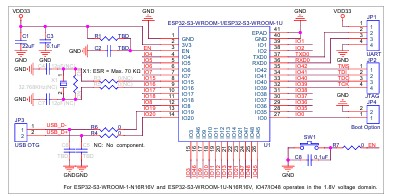
\includegraphics[width=0.7\linewidth]{../../../Images/Syde/Hypatia/EspPeripherals}
	\caption[Peripheral Schematics]{Peripheral Schematics \cite[see][42]{Espressif:2024}}
	\label{fig:EspPeripherals}
\end{figure}

\subsection{Electrical Characteristics}
The electrical characteristics define the operating limits, voltage levels, and current ratings required for reliable performance of the ESP32-S3 under various conditions.

\paragraph{Absolute Maximum Ratings}
Absolute maximum ratings define the limits beyond which permanent damage to the ESP32-S3 may occur. These ratings include the power supply voltage (VDD33), which must remain within -0.3\,V to 3.6\,V, and the storage temperature, limited to a range of -40$^\circ C$ to 105$^\circ C$. These values represent stress conditions only and functional operation outside the recommended range is not guaranteed and may affect long-term device reliability.

\paragraph{Recommended Operating Conditions}
Recommended operating conditions specify the voltage, current, and temperature ranges in which the ESP32-S3 is intended to operate reliably. The supply voltage (VDD33) should remain between -0.3\,V to 3.6\,V, with a typical value of 3.3\,V. The current (IVDD33) is defined as the current provided by the external power source. Operating temperature depends on the version: the -40$^\circ C$ to 85$^\circ C$ range applies to the standard version, while the extended temperature version supports up to 105$^\circ C$. Staying within these conditions ensures optimal device performance and longevity.

\paragraph{DC Characteristics }
The DC characteristics of the ESP32-S3 define the voltage and current levels required for proper digital input and output operation at a supply voltage of 3.3\,V and a temperature of 25$^\circ C$. Input thresholds are specified with a minimum high-level input voltage of 0.75 × VDD and a maximum low-level input voltage of 0.25 × VDD, ensuring reliable logic detection. Input leakage currents are minimal, with typical values below 50\,nA. Output levels are characterized by a high-level output voltage of at least 0.8 × VDD and a low-level output voltage not exceeding 0.1 × VDD when measured with a high-impedance load. Depending on the pad configuration, output drivers can source or sink up to 40\,mA and 28\,mA respectively. Internal weak pull-up and pull-down resistors are provided, with typical resistance values of $45\,\mathrm{k}\Omega$ and $25\,\mathrm{k}\Omega$. Reset pin behavior is also defined, with release and assertion thresholds consistent with standard digital logic levels, ensuring reliable device startup and shutdown conditions.

\paragraph{Current Consumption Characteristics}
Current consumption characteristics for the ESP32-S3 vary depending on the operating mode, supply voltage, and system configuration. In active mode with a 3.3\,V supply and ambient temperature of 25$^\circ C$, peak TX currents can range from 267\,mA to 355\,mA depending on the 802.11 protocol and data rate, while RX current remains under 100\,mA. In modem-sleep mode, current consumption is significantly reduced, with values depending on CPU frequency, core activity, and instruction set. Dual-core operation with 32-bit instructions shows the highest values, while single-core operation in idle state is considerably more efficient. At 240\,MHz, for example, dual-core execution of 128-bit instructions can draw up to 103.9\,mA.

In low-power modes, such as light-sleep or deep-sleep, typical current drops to the microamp range 8\,$\mu A$ for deep-sleep and 7\,$\mu A$ for hibernation. The chip can also be fully powered off by pulling the CHIP\_PU pin low, consuming just 1\,$\mu A$. It's important to note that for variants with embedded PSRAM, additional current must be considered depending on the memory size and operating voltage. For example, 8\,MB Octal PSRAM at 3.3\,V can add around 140\,$\mu A$, while 2\,MB Quad PSRAM at 3.3\,V adds approximately 40\,$\mu A$ in light-sleep mode. These measurements highlight the flexibility of the ESP32-S3’s power management, making it suitable for both high-performance and energy-constrained applications.

\subsection{RF Characteristics}
RF measurements are taken at the antenna port, where the RF cable is connected, and include losses from the front-end circuitry. For modules with external antenna connectors, the test setup uses antennas with a $50\Omega$ impedance. Devices are intended to operate within the center frequency ranges allocated by regional regulatory authorities. Both the target center frequency and the transmit power level can be configured through software, allowing adaptation to specific compliance and application requirements.

\subsubsection{Wi-Fi Radio}
Wi-Fi functionality on the ESP32-S3 is implemented according to the IEEE 802.11b/g/n standards and operates within a center frequency range of 2412\,MHz to 2484\,MHz. The transmit (TX) characteristics vary depending on the modulation and data rate. For example, typical transmit power reaches up to 20.5\,dBm for 802.11\,b at 1\,Mbps, while 802.11\,n using HT40 and MCS 7 operates at a typical 17.0\,dBm. Error Vector Magnitude (EVM) values are also provided for each mode, with stricter limits applied to higher data rates and modulation schemes. For instance, 802.11\,n HT40 at MCS 7 must meet an EVM limit of –27\,dB when transmitting at 17\,dBm. Receiver (RX) sensitivity is defined by a packet error rate (PER) of 8\% for 802.11\,b and 10\% for 802.11g/n. The RX sensitivity values indicate the minimum signal level required for reliable communication. At 1\,Mbps (802.11\,b), the receiver can detect signals as low as -98.2\,dBm, while for 802.11\,n HT40 at MCS 7, typical sensitivity is -71.2\,dBm. Maximum RX level values are also provided to indicate the strongest signal the receiver can tolerate without performance degradation, which remains consistently at 0 to 5\,dBm across data rates. The Adjacent channel rejection values for the ESP32-S3  vary depending on the modulation and data rate. At 802.11g with 6\,Mbps, the typical adjacent channel rejection is 35\,dB, while at higher-throughput modes such as 802.11\,n HT40 with MCS 7, the rejection decreases to around 8\,dB. 

\subsubsection{Bluetooth LE Radio}
Bluetooth LE functionality operates across a center frequency range of 2402\,MHz to 2480\,MHz, with a configurable RF transmit power ranging from -24.0\,dBm up to 20.0\,dBm. Transmitter characteristics are specified for various data rates including 1\,Mbps, 2\,Mbps, 500\,Kbps, and 125\,Kbps. Each configuration is defined by limits on carrier frequency offset and drift, modulation accuracy, and in-band spurious emissions. For instance, at 1\,Mbps, the carrier frequency offset must not exceed $/pm$150ß,kHz and modulation deviation must remain within -198.00\,kHz for 99.9\% of symbols. Spurious emissions are limited to -42\,dBm within $/pm$2\,MHz of the carrier and -44\,dBm beyond $/pm$3\,MHz.Receiver characteristics follow similar categorization per data rate. At 1\,Mbps, sensitivity is defined at –96.5\,dBm for a 30.8\% packet error rate. Co-channel and adjacent channel rejection values are listed for different frequency offsets, enabling assessment of interference tolerance. For example, at 2\,Mbps, co-channel interference rejection starts at 4\,dB for F = F0 $/pm$1\,MHz and increases to 8\,dB for F = F0 $/pm$2\,MHz. Adjacent channel selectivity and image frequency rejection are also provided, with values varying depending on signal spacing. These parameters allow evaluation of Bluetooth LE performance across different operating conditions. The available measurements collectively define transmitter accuracy, spectral containment, and receiver sensitivity—core factors that determine link stability and coexistence performance.

\section{\textcolor{red}{LSM100A}}%+Antenna
\section{Kommunikationsmodul LSM100A}

Das LSM100A stellt ein ultrakompaktes Funkmodul dar, das speziell für die Anforderungen des Internet der Dinge (IoT) entwickelt wurde. Die technische Besonderheit dieses Moduls liegt in seiner Hybrid-Architektur: Es vereint zwei der maßgeblichen LPWAN-Technologien (Low Power Wide Area Network) -- LoRaWAN und Sigfox -- auf einem einzigen Chip-System.

\subsection{Technische Kernaspekte und Funktionalität}
Ein zentrales Merkmal des LSM100A ist sein Dual-Mode-Betrieb. Das Modul ist in der Lage, sowohl innerhalb eines LoRaWAN-Netzwerks als auch über die Sigfox-Infrastruktur zu kommunizieren, wobei der Wechsel zwischen den Protokollen flexibel per Software oder über standardisierte AT-Befehle erfolgt. Technologisch basiert das Modul auf dem STM32WLE5-Chip von STMicroelectronics und wird in enger Kooperation mit dem Hersteller Seong Ji Industrial (SJI) gefertigt. 

Die Funkkommunikation findet im Sub-GHz-Bereich zwischen 863\,MHz und 928\,MHz statt, was insbesondere in Europa dem lizenzfreien ISM-Band entspricht. Trotz der sehr hohen Reichweite, die im freien Feld viele Kilometer abdecken kann, arbeitet das System mit einem minimalen Stromverbrauch. Diese Effizienz prädestiniert das Modul für den Einsatz in autarken, batteriebetriebenen Geräten, bei denen eine langfristige Wartungsfreiheit im Vordergrund steht.

\subsection{Physikalische Spezifikationen und Schnittstellen}
Mit einer Grundfläche von lediglich etwa 14\,mm $\times$ 15\,mm weist das LSM100A eine extrem kompakte Bauform auf, die eine Integration in platzkritische Hardware-Designs ermöglicht. Für die Anbindung externer Peripherie und Sensoren stellt das Modul eine Vielzahl an Schnittstellen zur Verfügung, darunter UART, SPI, I2C sowie analoge Eingänge (ADC) und universelle digitale Ein-/Ausgänge (GPIOs). 

Besonders hervorzuheben ist die Energieeffizienz im Betrieb: Im sogenannten Deep-Sleep-Modus reduziert sich die Stromaufnahme auf weniger als 2\,\textmu A, was theoretische Batterielaufzeiten von mehreren Jahren realisierbar macht. In der Standardausführung erfolgt die Steuerung des Moduls über eine serielle UART-Schnittstelle mittels einfacher AT-Befehle, was die Implementierung in bestehende Systemarchitekturen erheblich vereinfacht.

\section{Power Management}
The Hypatia Board features a USB-C interface \ref{fig:USBC}, which serves both as the primary power supply and as a means for uploading code to the ESP32 microcontroller. In addition, it includes a JST connector for attaching a battery, as well as a separate JST input for a solar panel, enabling the integration of an auxiliary power source and the ability to recharge the battery.

\subsection{USB-C Interface}
The board is equipped with a USB-C interface, which serves as both a power input and a data connection for programming and communication with the ESP32-S3 microcontroller. Through this single, compact connector, users can supply external 5V power to the system or interface with a host computer for firmware uploads, serial debugging, or data exchange.

\begin{figure}[H]
	\centering
	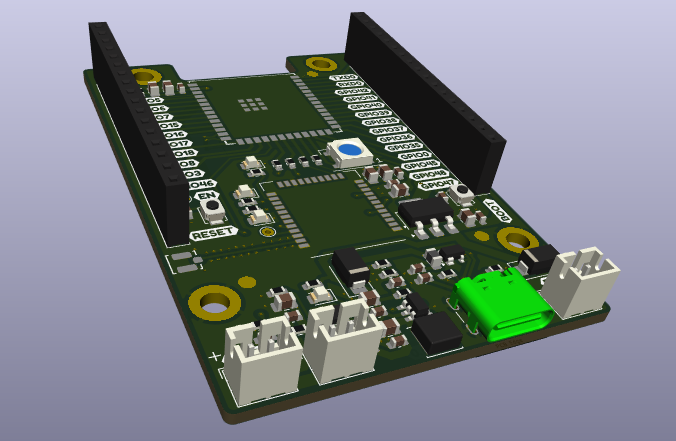
\includegraphics[width=0.3\linewidth]{../../../Images/Syde/Hypatia/USBC}
	\caption[USB-C Interface on Hypatia Board]{USB-C Interface on Hypatia Board}
	\label{fig:USBC}
\end{figure}

\begin{figure}[H]
	\centering
	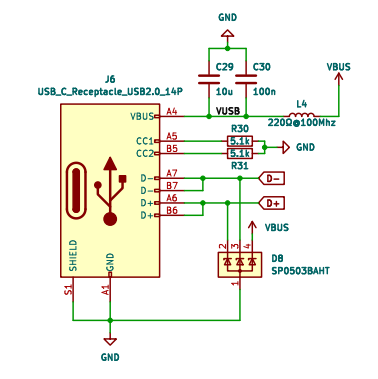
\includegraphics[width=0.3\linewidth]{../../../Images/Syde/Hypatia/USBCPlan}
	\caption[USB-C Interface on Hypatia Board Circuit diagram]{USB-C Interface on Hypatia Board Circuit diagram}
	\label{fig:USBCPlan}
\end{figure}

\subsubsection{SP0503BAHT TVS diode array }
To protect the system’s USB interface from electrostatic discharge (ESD) and transient voltage events, the SP0503BAHT TVS diode array \ref{fig:SP0503BAHT} is implemented between the USB-C connector and the internal circuitry. This component provides dedicated protection for the USB data lines (D+ and D-) as well as the VBUS supply line (+5V supply line in the USB port) \ref{fig:USBCPlan}. During events such as cable insertion or user interaction, the SP0503BAHT clamps sudden voltage spikes and diverts excess energy to ground. Its integration enhances for example the ESP32 microcontroller and other sensitive components from electrical overstress. \Mynote{SP0503BAHT Datasheet} 

\begin{figure}[H]
	\centering
	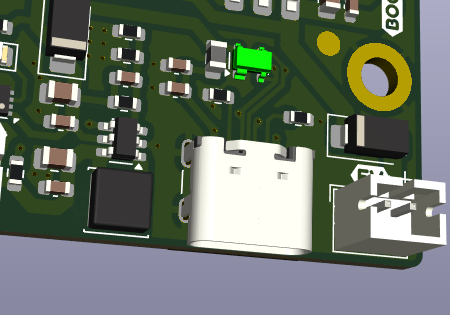
\includegraphics[width=0.3\linewidth]{../../../Images/Syde/Hypatia/SP0503BAHT}
	\caption[SP0503BAHT on Hypatia Board]{SP0503BAHT on Hypatia Board}
	\label{fig:SP0503BAHT}
\end{figure}


\subsubsection{SS14 Diode for USB-C Protection}
A SS14 Diode is integrated into the circuit to secure the power path from the USB-C input toward the charging controller. Its primary function is to prevent reverse current from flowing back into the USB power source.\Mynote{ Hypatia Datasheet} 

\begin{figure}[H]
	\centering
	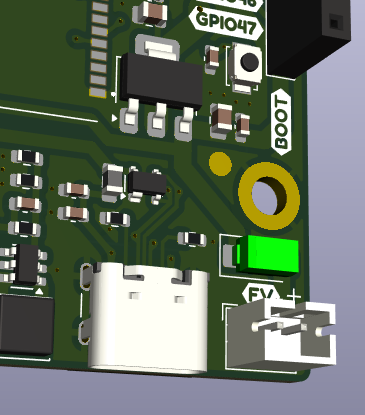
\includegraphics[width=0.3\linewidth]{../../../Images/Syde/Hypatia/SS14USBC}
	\caption[SS14 Diode for USB-C Interface on Hypatia Board]{SS14 Diode for USB-C Interface on Hypatia Board}
	\label{fig:SS14USBC}
\end{figure}

\subsection{Battery}
An external LiPo battery can be connected to the board via a dedicated JST connector \ref{fig:Battery}. The battery should provide a nominal output voltage of 3.7V, with a maximum fully charged voltage of 4.2V. When either a solar panel or a USB-C cable is simultaneously connected, the board is capable of recharging the battery. The battery begins to contribute meaningfully to the board’s power management system when its voltage exceeds 3.0V, which serves as the effective lower operational threshold. \Mynote{ Hypatia Datasheet} 

\begin{figure}[H]
	\centering
	
\includegraphics[width=0.3\linewidth]{../../../Images/Syde/Hypatia/Battery}
	\caption[Battery on Hypatia Board]{Battery on Hypatia Board}
	\label{fig:Battery}
\end{figure}

\subsubsection{Charger for Single-cell Li-Ion Batteries MC34673}
The charging process is managed by the MC34673 \ref{fig:MC34673}, a fully integrated single-cell Li-Ion/LiPo battery charger. When an external power source—such as a USB-C connection or a solar panel—is present, the MC34673 initiates a controlled multi-phase charging cycle. This includes an initial trickle charge phase for deeply discharged cells, followed by constant current (CC) charging for efficient energy delivery, and concluding with a constant voltage (CV) phase to safely reach the battery’s full charge capacity at 4.2V.

The charging current is configurable via an external resistor and is automatically adjusted through internal monitoring of voltage and thermal conditions. Built-in over-voltage protection (OVP), thermal foldback, and end-of-charge detection ensure both operational safety and longevity of the battery. Furthermore, when no power source is available, the MC34673 enters a low-power standby mode, drawing less than 1$\mu$A, thus preserving battery energy. In this architecture, the MC34673 functions as the system’s charging controller, coordinating power flow between sources and the energy storage component. \Mynote{Add Reference Datasheet}

\begin{figure}[H]
	\centering
	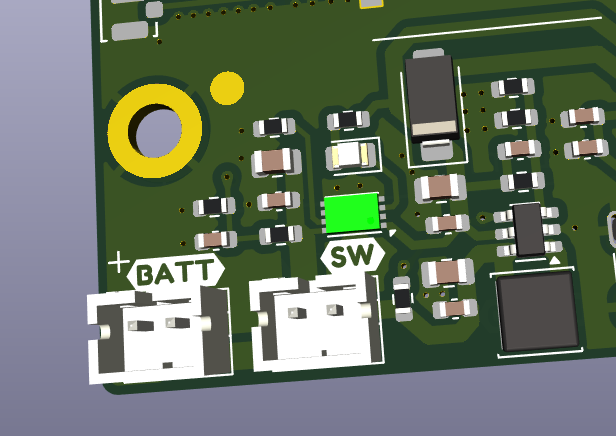
\includegraphics[width=0.3\linewidth]{../../../Images/Syde/Hypatia/MC34673}
	\caption[MC34673 on Hypatia Board]{MC34673 on Hypatia Board}
	\label{fig:MC34673}
\end{figure}

\subsubsection{Step-up Converter TLV61046ADB}
A TLV61046ADB step-up converter is implemented in the circuit \ref{fig:TLV61046ADB} to elevate the battery’s variable voltage to a stable 5V output. This regulated 5V rail is essential for powering downstream components that require a constant supply, regardless of the battery’s charge state. \Mynote{ Add Reference Datasheet}

\begin{figure}[H]
	\centering
	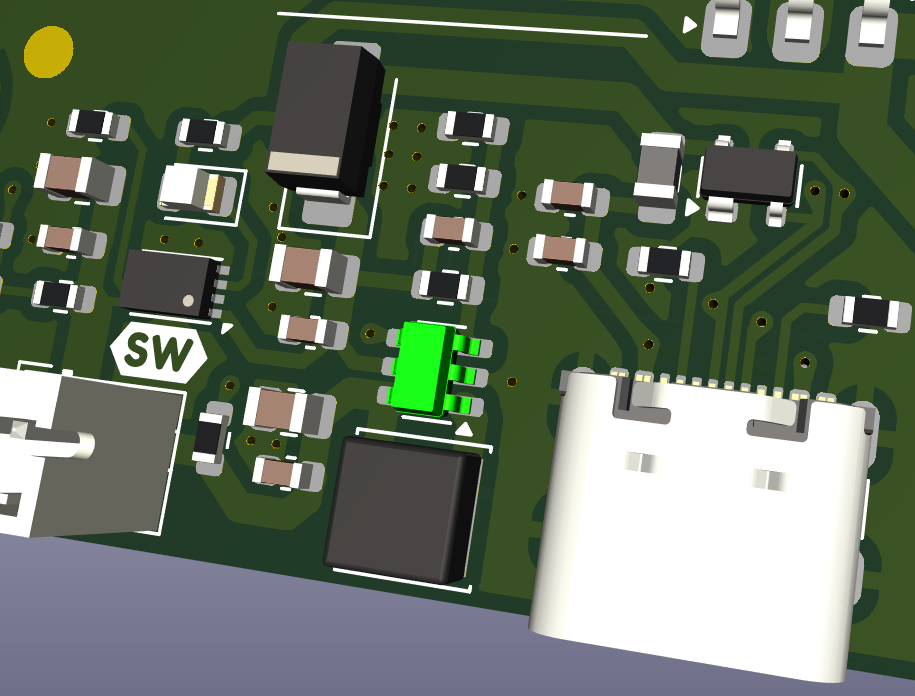
\includegraphics[width=0.3\linewidth]{../../../Images/Syde/Hypatia/TLV61046ADB}
	\caption[TLV61046ADB on Hypatia Board]{TLV61046ADB on Hypatia Board}
	\label{fig:TLV61046ADB}
\end{figure}

\subsubsection{AMS1117-3.3 linear voltage regulator}

To supply components that operate at lower voltages, the board integrates an AMS1117-3.3 linear voltage regulator \ref{fig:AMS1117}, which derives its input from the 5V rail generated by the TLV61046ADB boost converter. The AMS1117-3.3 provides a regulated 3.3V output, which is required by the ESP32-S3 microcontroller and other low-voltage peripherals.

\begin{figure}[H]
	\centering
	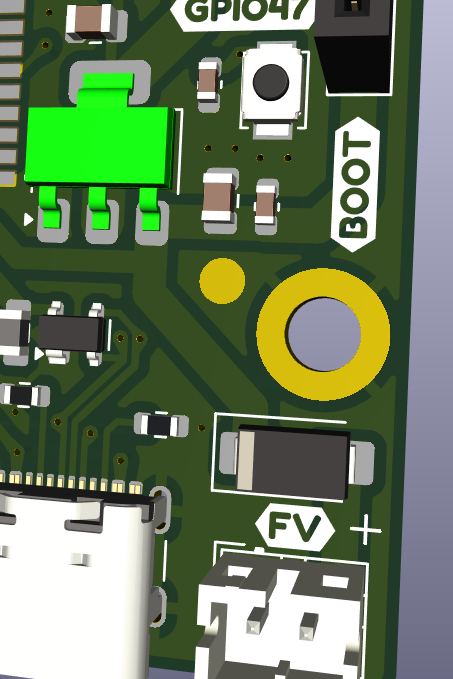
\includegraphics[width=0.3\linewidth]{../../../Images/Syde/Hypatia/AMS1117}
	\caption[AMS1117 on Hypatia Board]{AMS1117 on Hypatia Board}
	\label{fig:AMS1117}
\end{figure}

\subsubsection{Read battery Voltage Code Example}
A resistive voltage divider is implemented to monitor the battery voltage. The divider scales the voltage from the +BATT line down by a factor of 2, making it accessible through GPIO10. 




\definecolor{codegreen}{rgb}{0,0.6,0}
\definecolor{codegray}{rgb}{0.5,0.5,0.5}
\definecolor{codepurple}{rgb}{0.58,0,0.82}
\definecolor{backcolour}{rgb}{0.95,0.95,0.92}

\lstinputlisting[
caption= WiFi Check LED Code,
label={lst:WiFi cpp},
language=C++,
backgroundcolor=\color{backcolour},   
commentstyle=\color{codegreen},
keywordstyle=\color{magenta},
numberstyle=\tiny\color{codegray},
stringstyle=\color{codepurple},
basicstyle=\ttfamily\footnotesize,
breakatwhitespace=false,         
breaklines=true,                 
keepspaces=true,                 
numbers=left,       
numbersep=5pt,                  
showspaces=false,                
showstringspaces=false,
showtabs=false,                  
tabsize=2]{../../Code/Syde/HTADemonstrator/Test/VoltageReadBattery/VoltageReadBattery.ino}

\subsection{Solar panel}
An additional JST connector \ref{fig:SolarPanel} on the board allows for the integration of a solar panel as an alternative power source. This enables the system to harvest energy from ambient light, providing a supplementary supply to power the board and recharge the connected battery. 

\begin{figure}[H]
	\centering
	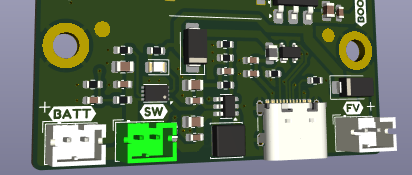
\includegraphics[width=0.3\linewidth]{../../../Images/Syde/Hypatia/SolarPanel}
	\caption[Solar Panel JST on Hypatia Board]{Solar Panel JST on Hypatia Board}
	\label{fig:SolarPanel}
\end{figure}

\subsubsection{SS14 Diode as Solar Panel Protection}
A SS14 diode is placed between the solar panel input and the charging circuit to ensure unidirectional current flow. This diode prevents reverse current from flowing back into the solar panel when it is inactive or exposed to low light conditions, thereby protecting the panel and enhancing the overall efficiency and reliability of the power management system. \Mynote{ Add Reference Datasheet}

\begin{figure}[H]
	\centering
	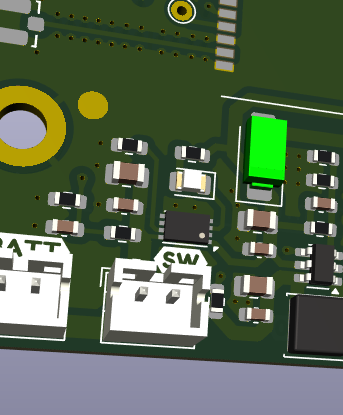
\includegraphics[width=0.3\linewidth]{../../../Images/Syde/Hypatia/SS14Solar}
	\caption[SS14 on Hypatia Board for Solar Panel]{SS14 on Hypatia Board for Solar Panel}
	\label{fig:SS14Solar}
\end{figure}














